\documentclass[final,a4paper,11pt,notitlepage,halfparskip]{scrreprt}

\usepackage[german,ngerman]{babel}
\usepackage[utf8]{inputenc}
\usepackage[T1]{fontenc}
\usepackage[babel,german=quotes]{csquotes}
%\usepackage{fancybox}
%\usepackage{color}
\usepackage{xcolor}
\usepackage{hyperref}
%\usepackage{floatflt}
\usepackage{graphicx}
%\usepackage{amsmath}
%\usepackage{amssymb}
%\usepackage{amsfonts}
%\usepackage{listings}

\setkomafont{caption}{\footnotesize\linespread{1}\selectfont}
\setlength{\abovecaptionskip}{-0.1cm}
\addto\captionsngerman{\renewcommand\figurename{Abb.}}

\title{Beleg\\
Rechnernetze/\\
Kommunikationssysteme}
\author{Jan Losinski}

\begin{document}

\maketitle

\tableofcontents

\chapter{Aufgabe}

\section{Wortlaut}\label{sec:aufgabe-wortlaut}
Schreiben Sie einen Daemon, welcher E-Mails per ESMTP annehmen und weiterleiten 
oder speichern sowie dem jeweiligen Nutzer per POP3 zur Verfügung stellen kann. 
Die Implementierung von ESMTP muss eine Authentisierung des Nutzers vor dem 
Absenden erzwingen. Die weitere Implementierung muss E-Mails annehmen und an die 
passende E-Mail-Domain weiterleiten können, falls es sich bei dem Empfänger 
nicht um einen lokalen Nutzer handelt. Das aussenden und Abrufen von E-Mails 
muss mit einem E-Mail-Programm, wie beispielsweise Evolution oder Thunderbird 
möglich sein.

Randbedingungen:
\begin{itemize}
  \item Implementierung in C, nicht C\# oder C++ oder \dots
  \item weitgehende Modularisierung, beispielsweise in einen POP3-Parser etc.
  \item der Daemon läuft als ein Prozess ohne Threads (oder Forks)
  \item das Mailboxformat darf beliebig sein
  \item das Mailboxformat darf beliebig sein
  \item die Anzahl der Nutzer darf auf 5 beschränkt sein
  \item der Daemon muss ohne weiteres auf den Rechnern im Labor S311 übersetzt 
        werden können und dort laufen
  \item Gruppenarbeiten sind nicht erlaubt
  \item Die Dokumentation des Daemons wie auch der Quellen geht in die Bewertung 
        ein
  \item es dürfen Bibliotheken verwendet werden, beispielsweise SQLITE oder 
        GDBM, soweit diese keine grundlegenden Funktionen von POP3 oder (E)SMTP 
	zur Verfügung stellen.
  \item Die Abgabe des Belegs erfolgt über das SVN. Geprüft wird die letzte 
        Revision. Das SVN ist ab 29.01.2009 0:00 nur noch lesbar. Nachreichungen 
	werden nicht akzeptiert.
\end{itemize}

Programmieren sie nicht einfach darauf los. Beginnen Sie mit einer Konzeption 
der benötigten Programmmodule. Diese Konzeption darf (und sollte auch) in 
Gruppenarbeit erstellt werden.

Der Daemon soll mindestend folgende Kommandozeilenparameter unterstützen
\begin{description}
  \item[-h] Dokumentation der Kommandozeilenparameter und exit
  \item[-V] Informationen zur Version, SVN-Revision und Autor (Name, Vorname, Login)
  \item[-p <Portnummer,Portnummer,Portnummer>] Portnummern mit Komma getrennt
            für (E)SMTP, POP3 und POP3S\\ 
            Voreingestellte Portnummern 25,110,995
  \item[-u <Dateiname>] Datei mit den Nutzernamen als CSV-Datei mit "`TAB"' als 
            Feld-Trenner\\ 
	    Format: \texttt{Login\textbackslash tPasswort\textbackslash
	    tsonstiges\dots\textbackslash n}
\end{description} 

\section{Erfragte Zusätze}
Folgende zusätzliche Fahten zur Aufgabenstellung wurden erfragt:
\begin{itemize}
  \item SMTPS soll nicht implementiert werden.
  \item Die Ein/Ausgabe kann blockierend erfolgen.
  \item Der Mailheader muss nicht geparst werden, auch eine Extraktion von
        Mail Adressen muss nicht erfolgen.
  \item Mailrelay soll nur bei authentifiziertem ESMTP möglich sein.
  \item Die Zustellung lokaler Mails ist ohne Authentifizierung möglich. 
  \item Die Implementation der Verschlüsselten Verbindung soll per SSL 
        erfolgen. STARTLS ist nicht gefordert.
\end{itemize}



\chapter{Umsetzung}
\section{Allgemein}\label{sec:umsetzung-allgemein}
Mit dieser Anwendung wurde ein rudimentärer Mailserver implementiert, welcher
SMTP und POP3 Funktionalitäten besitzt. Zudem besitzt er die Fähigkeit, über SSL
Verschlüsselte Verbindungen mit POP3 Clients zu sprechen.

Es gibt jedoch Einschränkungen, was die Geschwindigkeit und Sicherheit der 
Anwendung angeht, die durch die Aufgabenstellung bereits vorgegeben sind.
So werden alle Anfragen und Sitzungen in nur einem Thread abgehandelt. Es kann
also zu Verzögerungen kommen, wenn der Server z.B. gerade auf einen DNS 
Timeout wartet o.ä. Zudem wirken sich eventuelle Speicherüberläufe und 
Angriffe, welche diese ausnutzen auf den gesamten Server mit allen 
Verbindungen aus, da alle Sitzungen in nur einem Adressraum ablaufen.
Durch eine Aufteilung in unterschiedliche Adressräume durch \texttt{fork()}, 
wie es in vielen Mailservern praktiziert wird, könnte man dieses Problem lösen.
Zudem umgeht man damit das Problem der Verzögerung aller Verbindungen wenn eine
durch warten auf einen Timeout blockiert ist.

Da diese Implementation jedoch nur Beispielcharakter besitzen soll sind diese
Nachteile vertretbar. Es wird jedoch ausdrücklich darauf hingewiesen, das der
Server nicht für den Produktiveinsatz geeignet ist.


\section{Module}
Bei der Planung wurde festgestellt, das eine Aufteilung der funktionalen
Bestandteile des Programmes auf verschiedene getrennte und nur über definierte
Schnittstellen kommunizierende Module sinnvoll ist. So können Fehler lokal
begrenzt und schneller gefunden werden. Auch Seiteneffekte einer späteren 
Problembehebung können somit auf das bearbeitete Modul begrenzt werden, solang
die Schnittstelle zu den anderen Modulen gleich bleibt. 

Zudem wird der Code übersichtlicher und für dritte einfacher lesbar, da klar
definiert ist, wo nach einer bestimmten Funktionalität zu suchen ist.

Diese Modulaufteilung ist in C leider nur rudimentär umsetzbar, da es keine
echte Kapselung funktionaler Einheiten oder gar Namensräume gibt. Die Wahl einer
anderen Programmiersprache, wie z.B. C++ hätte dies wesentlich vereinfacht und
zusätzlich noch für besser lesbaren Code gesorgt. Auch die Typsicherheit und
eine damit einhergehende Reduzierung der Fehlerwahrscheinlichkeit in der
Implementation wären in vielen anderen Sprachen besser gewesen.

Die aus der Aufgabenstellung abgeleiteten Funktionalitäten, welche jeweils in
einem eigenständigem Modul zusammen gefasst sind zeigt die folgende Tabelle.
Zudem ist in Abb \ref{fig:schema} eine Übersicht über die Module und ihr
Zusammenspiel zu sehen.

Die Implementierungen der Module befinden sich jeweils in einer eigenen C-Datei,
welche den Namen des Moduls trägt. Die Schnittstellen sind in den gleichnamigen
Header-Dateien definiert.

\vspace{3mm}

\begin{tabular}[h]{lp{30em}}
  Modul       & Funktionalität \\
  \hline\hline
  config      & Hier geschieht die Konfiguration des Servers (auswerten der
                Kommandozeilen-Parameter) und die Bereitstellung der 
		Konfigurationsdaten für die anderen Module.\\
  connection  & Dieses Modul ist für alle Operationen zuständig die direkt mit
                der Verbindung zu tun haben. Dies ist das Annehmen neuer
		Verbindungen, das aufsetzen der listening Sockets, das Lesen der
		Daten vom Client, das Warten auf Daten von den Clients und das
		Schreiben von Daten zu den Clients.\\
  fail        & Ausgabe und Behandlung von Fehlern.\\
  forward     & Das forward Modul wird benutzt um eine Mail, welche nicht an
                eine lokale Mailbox ausgeliefert wird, an den betreffenden
		Mailserver weiterzuleiten.\\
  mailbox     & In diesem Modul sind alle Funktionen untergebracht, die zum
                lesen und schreiben der Mailboxen nötig sind. Auch
		Statusinformationen über eine Mailbox können hier abgefragt
		werden.\\
  main        & Dies ist das Start-Modul, in welchem die 
                \texttt{main()}-Funktion deklariert ist. Diese koordiniert die
		Initialisierungen, den Start der Hauptschleife sowie das
		Aufräumen am Programmende.\\
  pop3        & In diesem Modul sind alle Funktionen gekapselt, die zur
                Implementation des POP3 Protokolls benötigt werden.\\
  smtp        & In diesem Modul sind alle Funktionen gekapselt, die zur
                Implementation des SMTP/ESMTP Protokolls benötigt werden.\\
  ssl         & Dieses Modul dient zur Behandlung con SSL Verbindungen, welche
                für POP3S benötigt werden.\\
  \hline
\end{tabular}
\vspace{3mm}

Nachfolgend wird die Implementierung der einzelnen Module genauer beschrieben.
Dies wird über einen Groben Überblick jedoch nicht hinauskommen. Daher bitte ich
den Leser, bei konkreten Fragen zur Implementation die aus dem Code mittels
Doxygen generierte Dokumentation zur Hilfe zu nehmen. 


\subsection{Config}
Dieses Modul wird zum Start des Programms von der \texttt{main()}-Funktion
genutzt um die Kommandozeilen-Argumente zu parsen und zu verarbeiten. Dabei
werden intern Modul-globale variablen auf die per Kommandozeile übergebenen
Werte gesetzt. 

Zudem wird die CSV Datei mit den Nutzernamen und Passwörtern eingelesen und die
Daten in einer einfach gelinkten Liste abgelegt. Diese Liste speichert zudem den
Status der Mailbox des Nutzers (locked oder nicht). Der Name des Nutzers ist
gleichzeitig der Teil vor dem \texttt{@} seiner Emailadresse. Der Teil dahinter
setzt sich aus dem per Kommandozeile angegebenem Hostnamen zusammen. Ist kein
Hostname angegeben, so besitzt der Nutzer \texttt{<Nutzername>@localhost} als
Emailadresse.

Die in diesem Modul gespeicherten Werte können über klare Schnittstellen, welche
in der Headerdatei definiert sind, jederzeit von anderen Modulen abgefragt
werden.

Das Modul besitzt außerdem Funktionen zum Prüfen, ob ein Nutzer existiert, ob
ein Passwort korrekt ist und ob die Mailbox des Nutzers grad gesperrt ist oder
nicht.


\subsection{Mailbox}
Im Mailbox Modul ist, wie der Name schon sagt, alles implementiert, was für die
lokalen Mailboxen von Nöten ist. Die Mailboxen selbst sind mittels SQLITE
realisiert. Dazu besteht eine SQLITE Datenbank-Datei, in welcher eine Tabelle
Existiert. In dieser Tabelle werden alle Mails mit dem Nutzernamen, dem die
Mailbox gehört, sowie einem eindeutigem Bezeichner (eine Zahl, welche bei jeder
neuen Mail um eins erhöht wird) und der Größe der Mail abgelegt.

Diese Ablage in einer SQLITE Datenbank hat den Vorteil, das man sich um die
Zuordnungen der Mails zur jeweiligen Mailbox, um das Lesen und Schreiben der
Dateien, um das generieren einer ID und vieles mehr keine Gedanken weiter machen
muss. Man kann einfach mit Standard-SQL Abfragen arbeiten und bekommt immer die
korrekten Daten geliefert - die SQLITE Bibliothek kümmert sich um den Rest.
Performancenachteile wurden nicht festgestellt, zumal eine eigene
Implementierung dieser Funktionalitäten aufgrund der kurzen Zeit sicher nicht
optimal wären.

Das Mailbox Modul muss zu beginn des Programmes initialisiert werden, um eine
ordnungsgemäße "`Verbindung"' zur Datenbank-Datei aufbauen zu können. Am ende der
Anwendung ist dann ein de-initialisieren nötig, um die Datei wieder zu
schliessen.

Nach der Initialisierung des Moduls können nach belieben neue Emails in die
Mailboxen geschrieben werden. Dazu dient lediglich die Funktion
\texttt{mbox\_push\_mail()}, welche alle relevanten Daten als Argumente
übergeben bekommt.

Zum Auslesen von Emails, bzw. Extraktion von Metadaten ist ein weiterer Schritt
der Mailbox-Initialisierung notwendig. Zu jeder Mailbox sollte jeweils nur
maximal ein initialisiertes Exemplar bestehen, da bei der Initialisierung alle
Metadaten der Mailbox eingelesen und während der Benutzung nicht mehr
aktualisiert werden. Gibt es zu einer Mailbox gleichzeitig zwei initialisierte
Instanzen kann es zu Inkonsistenzen kommen, welche Programmfehler verursachen.
Dies ist jedoch ein vertretbarer Nachteil, da das Zugreifende Modul (POP3)
mittels locking nur eine Verbindung pro Nutzer zu einer bestimmten Zeit zulässt.
Dies ist notwendig, da das Protokoll (rfc1939) es so vorsieht.

Bei der Initialisierung wird eine neue \texttt{mail}-Struktur erstellt und mit
Daten gefüllt. Dies ist unter anderem eine Liste mit Zuordnungen, welche jeder
Mail mit ihrem eindeutigem Bezeichner eine fortlaufende Nummer in der Mailbox
zuordnet. Über diese Nummern kann anschließend über die Schnittstellen auf
bestimmte Mails zugegriffen werden. Dies ist notwendig, da die Mails in einer
POP3 Mailbox durchnummeriert sind und die Zählung bei 1 beginnt. Zusätzlich wird
zu jeder Mail die Größe gespeichert welche aufaddiert in der Struktur noch als
Gesamtgröße gespeichert werden.

Ist diese Initialisierung abgeschlossen kann über die Schnittstellen auf die
Emails in der Mailbox, sowie deren Metadaten zugegriffen werden. Beim Löschen der
Mails ist zu beachten, das dies, wie im POP3 Protokoll benötigt, nicht sofort
geschieht. Die betreffenden Mails bekommen in der oben genannten Liste vorerst
nur eine Markierung, das sie zum Löschen vorgesehen sind. erst beim
de-initialisieren (Schließen) der Mailbox können diese gelöscht werden.
Zusätzlich können die Löschmarkierungen jederzeit zurückgesetzt werden.

Nach der Benutzung einer Mailbox muss diese wieder de-initialisiert (geschlossen
werden. Die Funktion zur De-Initialisierung (mbox\_close()) besitzt ein Flag als
Argument (has\_quit), welches anzeigt, ob die Mailbox ordnungsgemäß geschlossen
werden soll oder nur de-initialisiert. Beim ordnungsgemäßen Schließen werden im
Gegensatz zum einfachen de-initialisieren alle als gelöscht markierten Emails 
aus der Datenbank gelöscht.


\subsection{Connection}
Dieses Modul ist das Zentralste in der ganzen Anwendung. Es verwaltet Alle
Verbindungen und verteilt die empfangenen Daten. Zum Start der Anwendung muss
auch dieses Modul initialisiert werden. Dabei werden die drei Listening-Sockets,
welche auf den angegebenen Ports auf Client Verbindungen warten geöffnet und
gebunden. Die Verbindungen werden jeweils in einer \texttt{mysocket}-Struktur
gekapselt. In dieser Struktur befinden sich alle Daten die zu der jeweilige
Verbindung gehören. Dies sind verschiedene Callback-Funktionen zum Verarbeiten
der Daten und die Daten der selbst. Die Daten einer Verbindung sind in erster
Linie die Session Strukturen der Client Verbindungen, welche zum Beispiel den
Status einer SMTP Verbindung oder die Mailbox einer POP3 Verbindung enthalten.

Die \texttt{mysocket}-Strukturen werden in einer einfach gelinkten Liste
gespeichert. In der Hauptschleife des Programms, welche auf Daten von den
Clients oder neue Verbindungen wartet, werden alle Dateidescriptoren aus der
Liste der Verbindungen in ein \texttt{fd\_set} geschrieben und einem
\texttt{select()} übergeben. Kehrt das \texttt{select()} zurück wird die Liste
erneut durchlaufen und für jede Verbindung, die Daten bereit hält die
entsprechende Callback-Funktion aufgerufen.

Diese Funktionen lesen dann je nach Verbindungstyp Daten vom Client und
übergeben diese an das entsprechende Modul oder akzeptieren eine neue Verbindung
und initialisieren diese.
Beim lesen der Daten ist zu beachten, das diese nach Zeilen getrennt an die
entsprechenden Module übergeben werden. Bei SSL Verbindungen wiederum wird das
SSL Modul benutzt um die Daten zu lesen, bzw. nach einem erfolgreichem 
\texttt{accept()} einer neuen Verbindung der SSL Handshake durchgeführt.

Die Module an die die gelesenen Daten übergeben werden sind das Pop3-, das 
Smtp- und das Forward-Modul. Diese Funktionen sind in der \texttt{mysocket}
Struktur entsprechend als Callback Funktion gesetzt.

Die Module Pop3 und Smtp besitzen zudem noch Funktionen zum initialisieren neu
akzeptierter Verbindungen. Dabei werden die Sitzungsdaten, welche für das 
Jeweilige Protokoll benötigt werden initialisiert. Diese Funktionen sind als 
Callback-Funktionen der jeweiligen Listening-Verbindung gesetzt, so das sie 
automatisiert aufgerufen werden können wenn eine neue Verbindung entsteht.

Beim Schließen von Verbindungen wird die zugeordnete Callback-Funktion der
Verbindung zum Aufräumen der Sitzungsdaten aufgerufen. Diese sind ebenfalls in
den drei Modulen Pop3, Smtp und Forward definiert. Dieser Aufruf passiert in der
Funktion, welche die \texttt{mysocket}-Strukturen aus der Liste der Sockets
entfernt und die Sockets schliesst (\texttt{conn\_delete\_socket\_elem()}).
Sollte die Verbindung eine SSL Verbindung sein, so wird hier auch die SSL
Verbindung ordnungsgemäß abgebaut.

Für das Forward Modul existieren zudem Funktionen zum Aufbauen neuer Verbindungen
zu einem weiterem Mailserver oder einem Mailrelay. Diese neuen Verbindungen
werden anschließend wie normale Client Verbindungen in die Liste der Sockets
eingereiht.

Am Ende des Programmes wird von \texttt{main()} die Funktion 
\texttt{conn\_close()} aufgerufen. Diese wird auch als Signalhandler für alle
Signale die ein Ende des Programmes andeuten gesetzt. Sie geht die Liste der
Sockes durch und baut alle Verbindungen ordnungsgemäß ab.


\subsection{Smtp}
Dieses Modul implementiert das SMTP (rfc 5321) Protokoll mit einigen ESMTP 
Erweiterungen. Normale SMTP Sitzungen werden mit \texttt{HELO} Eingeleitet und
sind auf das ausliefern von Emails an lokale Mailboxen begrenzt. Jeder Versuch
eine Email an eine nicht-lokale Adresse zu senden wird mit einem Fehler
quittiert. ESMTP Sitzungen werden mit einem \texttt{EHLO} des Clients
eingeleitet. ESMTP Sitzungen müssen stets Authentifiziert werden. In
Authentifizierten ESMTP Sitzungen können auch Emails an nicht-lokale Adressen
versandt werden. Diese werden dann mittels des Forward-Moduls an den betreffenden
Mailserver oder einen angegebenen Relayhost weitergeleitet.

Da SMTP/ESMTP Sitzungen stark Statusbehaftet sind muss in der Sitzungsstruktur,
welche nach einem \texttt{accept()} einer neuen Verbindung initialisiert wird
gespeichert werden. Anhand dieses Status wird der aktuelle Input des Clients
verarbeitet und je nach Ergebnis ein Replycode gesendet sowie ein neuer Status 
gesetzt oder nicht. Die Sitzungsstruktur wird dabei automatisch bei der
Verarbeitung der Eingaben gefüllt und wieder geleert.

Die Authentifizierung geschieht per \texttt{AUTH PLAIN}, welches der einzige
implementierte Authentifizierungsmechanismus ist. Bei \texttt{AUTH PLAIN}
schickt der Cient lt. Standard nach einem \texttt{AUTH PLAIN} einen Base64
kodierten String von der Form:\\
\texttt{<Nutzerid>\textbackslash0<Nutzername\textbackslash0<Passwort>}. 
Interessant für die Authentifizierung ist dabei der Nutzername und das Passwort.
Mittels des Config Moduls wird zuerst geprüft, ob der Nutzer existiert und
anschließend ob das Passwort korrekt ist. Ist beides Erfolgreich, so wird die
Sitzung als Authentifiziert markiert. Die Dekodierung des Strings wird von der
SSL Bibliothek übernommen.

Der Emailclient Mozilla Thunderbird hält sich leider nicht an den Standard und
sendet \texttt{AUTH PLAIN} und des String mit den Nutzerdaten in einer Zeile.
Dies machte eine Ausnahmebehandlung notwendig, in welcher überprüft wird, ob die
Eingabe, in der \texttt{AUTH PLAIN} erwartet wird länger ist als der String
\texttt{"`AUTH PLAIN"'}. Ist dies der Fall, so wird angenommen, das danach die
Nutzerdaten folgen. Die Eingabe nach dem \texttt{AUTH PLAIN} plus ein
Leerzeichen wird also an die Funktion zum Überprüfen der Nutzerdaten übergeben.

Die Steuerkommandos des SMTP Protokolls werden stets Case-Insensitiv überprüft.
Zudem werden bei Kommandos mit Argumenten die Leerzeichen zwischen dem Kommando
und dem Argument entfernt. Schlägt die Überprüfung eines erwarteten Kommandos
fehl, so wird geprüft ob eines der wahlfrei in der Sitzung verwendbaren
Kommandos (z.b. \texttt{RSET}, \texttt{QUIT} oder \texttt{NOOP}). aufgetreten
sind und werden bei Auftreten entsprechend behandelt.

Die in der Sitzung angegebenen Emailadressen für den Empfänger und den Absender
werden direkt nach dem jeweiligen Empfang geprüft. Geprüft wird, ob der Teil vor
dem @ mindestens 2 Zeichen lang ist und ob der Teil nach dem @ ein existierender
Hostname ist oder es einen MX Record dazu gibt. 

Bei den Empfängeradressen wird zudem geprüft, ob die Adresse lokal existiert.
Ist dies der Fall, so wird die Email nach der Annahme an die entsprechende
lokale Mailbox ausgeliefert. Ist die Adresse nicht-lokal, so wird die Email an
das Forward Modul übergeben, welches sie an den entsprechenden Mailserver
weiterleitet.

Die MX Records zu den Emailadressen werden von dem Resolver der libc aufgelöst.
Dies hat den Vorteil, das keine weiteren Bibliotheken auf dem System vorhanden
sein müssen. Leider ist dieser Teil der Bibliothek nicht gut dokumentiert, so
das zur Implementation der MX-Record-Auflösefunktion der Code des ClamAV
Virenscanners als Beispiel zur Hilfe genommen wurde. Der resultierende Code
sieht auf den ersten Blick etwas kompliziert aus, dies liegt jedoch nur an der
komplizierten Verarbeitung eines Auflöseresultats. Die Funktion ermittelt
lediglich den ersten MX Record zu einem namen. Dies sollte in der Regel
ausreichen. Sonst möchte ich an dieser Stelle auf den Beispielcharakter der
Anwendung hinweisen, welcher explizit gefordert wurde.

Der eigentliche Datenblock der Mail wird Zeilenweise eingelesen und in einer
einfach gelinkten Liste abgelegt. Dies hat den Vorteil, das kein kompliziertes
Speichermanagement notwendig ist, obwohl man zu Beginn noch nicht weiß wie groß
der momentane Datenblock wird. Vor dem lokalem Ausliefern werden dann alle 
Zeilen in einen einzigen Speicherblock geschrieben. Dies ist relativ einfach, 
da zu jedem Zeilenelement in der Liste die Länge der Zeile gespeichert wird. 
Es muss also nur durch die Liste iteriert, die Größen addiert und ein 
Speicherblock mit der entsprechenden Größe allokiert werden. 
Anschließend wird erneut über die Liste iteriert und die einzelnen Zeilendaten 
mittels \texttt{memcpy()} in den Puffer kopiert. Auch hier ist die jeweils zu der 
Zeile gespeicherte Länge wieder hilfreich, da so der Offset für das Kopieren 
einfach durch Addition der Längen zu berechnen ist. 
An das Forward Modul zum weiterleiten der Email wird die komplette Zeilenliste
übergeben.
Beendet wird der Datenblock wie im Standard beschrieben mit
\texttt{<CR><LF>.<CR><LF>}. Wird diese Sequenz gefunden wird die Annahme der
Daten beendet und die Mail sofort an das Forward Modul übergeben oder lokal
ausgeliefert.

Nach der Auslieferung oder Weiterleitung einer Mail wird die Sitzungsstruktur
sofort wieder bereinigt und kann eine weitere Email entgegen nehmen. Beendet
wird die Sitzung mit einem \texttt{QUIT} des Clients. Nach einem \texttt{QUIT} 
baut das Connection Modul die Verbindung ab und lässt das SMTP Modul mit Hilfe 
der Aufräum-Callback-Funktion die Sitzungsstruktur leeren und freigeben.


\subsection{Forward}
Das Forward Modul dient der Weiterleitung einer Email. Es bekommt Emails vom
SMTP Modul übergeben, welche nicht lokal ausgeliefert werden können. Der
Datenblock wird als eine Liste von Zeilen übergeben, welche das Modul in seine
eigene \texttt{fwd\_mail}-Struktur kopiert, damit es nach dem Freigeben des
Speichers in dem SMTP Modul nicht zu Problemen kommt.

Noch vor dem Kopieren wird jedoch der Host ermittelt, an welchen die Email
weitergeleitet werden soll und mittels \texttt{conn\_new\_fwd\_socket()} aus dem
Connection Modul eine Verbindung zu diesem aufgebaut. Zudem reiht diese Funktion
die neu generierte Verbindung in die Socketliste des Connection Moduls ein und
setzt die nötigen Callback-Funktionen.

Wenn die Verbindung aufgebaut und \texttt{fwd\_mail}-Struktur initialisiert ist,
ist die Übergabe an das Forward Modul abgeschlossen. Die weiteren Aktivitäten
werden durch Eingaben des Clients gesteuert, welche durch das Connection Modul
an das Forward Modul übergeben werden.

Da das Forward Modul, wie das SMTP Modul ebenfalls eine SMTP Sitzung
durchführt, muss auch dieses den Momentanen Status der Verbindung speichern.
Dies geschieht in der bereits angesprochenen \texttt{fwd\_mail}-Struktur. Das
jeweils zu Sendende Kommando wird dann aus dem aktuellen Status und dem letzten
Replycode des Mailservers, an den die Email weitergeleitet werden soll,
bestimmt.

Kommt es zu einem Fehler, welcher sich nicht einfach durch erneutes Senden der
letzten Nachricht beheben lässt, so wird der Sendevorgang abgebrochen und eine
Email mit der Fehlernachricht und dem Inhalt der Originalemail an den Absender
verschickt. Die Funktion zum Weiterleiten einer Email hat dabei ein Argument
namens \texttt{failable}, welches anzeigt, ob diese eben genannte Mail versendet
werden soll oder nicht. Dies ist notwendig, damit es nicht zu einer Fehleremail
auf einen fehlgeschlagenen Sendevorgang einer Fehleremail kommt.

Nach einem Sendevorgang wird ein \texttt{QUIT} an den Mailserver gesendet und
gewartet, das das Connection Modul die Verbindung abbaut und die
\texttt{fwd\_mail}-Struktur aus dem Speicher bereinigt.


\subsection{Pop3}\label{sec:umsetzung-pop3}
Im Pop3 Modul ist, wie der Name schon sagt, das Pop3 Protokoll (rfc1939)
implementiert. Über das Pop3 Protokoll kann ein Client die Emails aus einer
lokalen Mailbox abrufen sowie sich Metadaten dazu anzeigen lassen.

Eine Pop3 Sitzung muss immer Authentifiziert werden, da sie immer mit der
Mailbox eines bestimmten Nutzers arbeitet. Zudem ist eine Pop3 Sitzung in drei
Abschnitte unterteilt, welche durch einen Status repräsentiert werden. Die drei
Zustände sind:
\begin{description}
    \item[\texttt{AUTH}] Repräsentiert eine nicht-authentifizierte Sitzung.
    \item[\texttt{START}] Repräsentiert eine laufende authentifizierte Sitzung.
    \item[\texttt{QUIT}] Repräsentiert eine beendete Sitzung.	
\end{description}
Alle Zustände sowie die Mailbox- und Nutzer-Daten werden in einer
\texttt{pop3\_session}-Struktur gespeichert und stehen damit über die gesamte
Sitzung zur Verfügung. 

Zur Authentifizierung sendet der Client zu Beginn seiner Sitzung die zwei 
Kommandos \texttt{USER <Nutzername>} und \texttt{PASS <Passwort>} senden muss.
Nach Empfang des Nutzernamens wird dieser mit Hilfe des Config Moduls geprüft. 
Wenn er existiert wird eine Positive Antwort gesendet. Anschließend wird 
geprüft, ob das Passwort valide ist. War diese Prüfung erfolgreich, so wird 
versucht die Mailbox des Nutzers zu sperren. Das heißt, es wird in der 
Nutzerliste des Config Moduls das Sperrflag des Nutzers gesetzt. Dies ist 
nötig, da die Pop3 Implementierung nur eine gleichzeitige Sitzung erlaubt. 
War das Prüfen und Sperren erfolgreich, wird eine positive Antwort gesendet und
der \texttt{START} Status gesetzt.
Alle Kommandos die nicht im rfc1939 im AUTHORIZATION State definiert sind und
nicht \texttt{USER} oder \texttt{PASS} sind werden mit einem \texttt{-ERR}
quittiert.

Im \texttt{START} Status kann der Client wahlfrei alle Kommandos benutzen,
welche laut rfc1939 als Mindestanforderung definiert sind. Zusätzlich wurde das
optionale Kommando \texttt{UIDL} Implementiert, da ohne \texttt{UIDL} oder
\texttt{TOP} der Emailclient Mozilla Thunderbird nicht in der Lage ist Emails
mit dem vorliegendem Programm abzurufen. Alle anderen, nicht implementierten
Kommandos werden mit einem einfachem \texttt{-ERR} Quittiert. 

Die Implementierungen der einzelnen Kommandos wurden so umgesetzt, das sie den
Standard rfc1939 so gut wie möglich umsetzen. Für Details zur Funktionsweise
oder Benutzung der einzelnen Kommandos möchte ich daher auf den Standard 
rfc1939 verweisen.

Der \texttt{QUIT} Zustand zeigt an, das die Sitzung beendet wurde. Er wird nur
zwischen einem \texttt{QUIT} des Clients und dem Abbau der Verbindung
angenommen. Nach einem ordnungsgemäßem \texttt{QUIT} werden alle zum Löschen
markierten Emails der Mailbox gelöscht. Dem Connection Modul wird mitgeteilt,
das es die Verbindung abbauen und die Callback-Funktion zum Aufräumen der
\texttt{pop3\_session}-Struktur aufrufen kann.

Die möglichen Kommandos der einzelnen Zustände sind als Array von
\texttt{pop3\_command}-Strukturen abgelegt. Diese Strukturen bestehen immer aus
einem Kommando, einer aufzurufenden Funktion und einem Flag, ob für die Funktion
ein Argument aus der Nachricht des Clients extrahiert werden soll oder nicht.
Das letzte Element dieser Arrays besteht immer aus \texttt{NULL}. Dies hat den 
Vorteil, das zum Parsen des Kommandos nur das Array durchlaufen und die 
Kommandos mit der Nachricht des Clients verglichen werden müssen. Wurde eine
Übereinstimmung festgestellt kann die zugeordnete Funktion direkt aufgerufen
werden.

Für das Schreiben der Antworten zum Client wird beim Initialisieren der
\texttt{pop3\_session}-Struktur eine extra Callback-Funktion aus dem Connection
Modul gesetzt. Dies ist nötig, da so transparent SSL und nicht-SSL Verbindungen
bedient werden können. Mit diesem Vorgehen könnte auch das Smtp Modul problemlos
um SmtpS Funktionalitäten erweitert werden.


\subsection{Ssl}
Das Ssl Modul stellt alle Funktionen zur Kommunikation mit Clients über eine SSL
Verbindung bereit. Es arbeitet vollkommen unabhängig vom verwendetem
Anwendungsprotokoll. Die Konfigurationen, wie der Name der Zertifikastdatei, etc
stehen momentan fest im Code. Dies ist mit der vorhandenen Infrastruktur des
Config Moduls bei Bedarf problemlos als Kommandozeilen-Option umsetzbar. Für
diese Anwendung mit Beispielcharakter soll die feste Codierung jedoch genügen.

Zu Beginn der Anwendung muss das Ssl Modul initialisiert werden. Dabei wird ein
SSL-Kontext (\texttt{SSL\_CTX}) erstellt und mit den richtigen Optionen
initialisiert. Dies minimiert den Aufwand bei späteren SSL Verbindungen, bei
denen lediglich der einmal erstellte Kontext benutzt wird.

Ist der Kontext initialisiert können neue Client Verbindungen durch einen SSL
Handshake aufgebaut werden. Dies geschieht durch die Funktion
\texttt{ssl\_accept\_client()}, welche lediglich einen Dateidescriptor bekommt,
welcher den Socket zum Client darstellt. Zurückgegeben wird ein Pointer auf eine
\texttt{SSL}-Struktur. Diese wird im späterem Verlauf der Verbindung benötigt um
Daten vom Client zu lesen oder zu ihm zu senden.

Das Lesen und Senden von Daten geschieht über die Funktionen \texttt{ssl\_read()}
sowie \texttt{ssl\_write()}. Diese werden ähnlich wie die libc Funktionen
\texttt{read()} und \texttt{write()} aufgerufen, bekommen jedoch immer den
zugeordneten \texttt{SSL}-Struktur-Pointer. Auch die Rückgabewerte der Funktionen
sind ähnlich der der libc Funktionen.

Am Ende einer SSL Verbindung muss zusätzlich zum normalen \texttt{close()} noch
ein \\
\texttt{ssl\_quit\_client()} aufgerufen werden, um (vor dem \texttt{close()}) die 
SSL Verbindung ordnungsgemäß zu beenden. Dies wird durch das 
\texttt{socket\_is\_ssl} Flag in der \texttt{mysocket} Struktur der Verbindung
im Connection Modul realisiert. Dieses Flag wird von der Funktion, welche im
Connection Modul für das Abbauen von Verbindungen zuständig ist ausgewertet.
Wenn die gesamte Anwendung beendet wird muss der SSL Kontext mit
\texttt{ssl\_app\_destroy()} wieder aufgeräumt werden. 



\chapter{Benutzung}

\section{Allgemein}
Das vorliegende Programm kann als rudimentärer Mailserver verwendet werden.
Dabei implementiert es die Funktionalitäten eines Mailservers, eines Mailrelays
und eines POP3 Servers, welcher zusätzlich noch SSL-verschlüsselte Verbindungen
beherrscht. Es gelten jedoch einige Aufgabenbedingte Einschränkungen, welche
unter \ref{sec:umsetzung-allgemein} aufgeführt sind.

Die SMTP Implementierung besitzt zudem einige Besonderheiten. So ist mit einer
normalen SMTP Sitzung (eingeleitet mit einem \texttt{HELO} des Clients) nur das
ausliefern von Emails an lokale Adressen möglich. Um eine Email an eine
nicht-lokale Adresse zu versenden muss der Client das erweiterte SMTP Protokoll
ESMTP (eingeleitet mit einem \texttt{EHLO} des Clients) benutzen. ESMTP
Sitzungen müssen jedoch immer mit Nutzername und Passwort Authentifiziert
werden. Die Nutzername-Passwort-Kombinationen stehen in einer Datei, welche beim
Start der Anwendung als Kommandozeilen-Option angegeben wird. Das Format dieser
Datei hält sich an die Vorgabe in der Aufgabenstellung (siehe
\ref{sec:aufgabe-wortlaut}). 

Nach erfolgreicher Authentifizierung per \texttt{AUTH PLAIN} ist auch ein
Versandt an nicht-lokale Adressen möglich. Dazu kann beim Starten des Programmes
ein Relayhost angegeben werden. Ist diese Option angegeben, werden alle Emails
die nicht lokal ausgeliefert werden können an diesen Server versandt. Ohne diese
Option werden die Emails an den Server gesandt, welcher durch den Teil nach dem
@ der Email bezeichnet wird oder an den MX Host dieses Bezeichners.

Die lokalen Email-Konten werden durch die Nutzer, welcher in der oben genannten
Datei spezifiziert sind und dem Hostnamen des Servers zusammengesetzt. Der
Nutzername ergibt dabei den Zeil vor dem @, der Hostname den danach. Beim Start
der Anwendung kann der Hostname als Kommandozeilen-Option übergeben werden. Der
Server versucht sich dann an diese Adresse zu binden. Wird kein Hostname
angegeben, so wird \texttt{localhost} als Hostname angenommen und der Server
bindet sich an \texttt{INET\_ANY}, d.h. an alle lokalen Netzwerkinterfaces.

Die Emails der lokalen Konten können per POP3 vom vorliegendem Server abgeholt
werden. Dabei werden alle notwendigen POP3 Kommandos und die optionalen
Kommandos \texttt{UIDL}, \texttt{USER} und \texttt{PASS} unterstützt.
POP3-Sitzungen müssen immer Authentifiziert werden. Dies geschieht per Klartext
\texttt{USER}$\rightarrow$\texttt{PASS} Sequenz. Als Nutzerdaten gelten ebenfalls
die Daten in der oben genannten Datei. In den Mailboxen gespeicherte Emails
bleiben auch nach dem Programmende erhalten. Es ist nur eine POP3 Verbindung pro
Nutzer und Zeitraum möglich. Der Versuch eine zweite Verbindung zu öffnen wird
mit einem Fehler quittiert (siehe \ref{sec:umsetzung-pop3}).

Das POP3 Protokoll kann auch durch eine SSL Verschlüsselte Verbindung genutzt
werden. Dazu muss sich der Client lediglich zu dem dafür eingestellten Port
verbinden. Das Zertifikat ist selbst-signiert und liegt im Wurzelverzeichnis des
Servers.

Alle oben genannten Funktionalitäten sind mit dem Emailclient Mozilla
Thunderbird in der Version 2.0.0.19 erfolgreich getestet. Zudem wurde die
korrekte Funktion nach den entsprechenden RFCs per Telnet sowie Openssl-Client
erfolgreich getestet. Durch die Standardnahe Umsetzung kann die genau
Funktionsweise der Protokolle in den entsprechenden RFCs nachgelesen und muss
hier nicht weiter besprochen werden.

Das Programm gibt Status und Fehlermeldungen während der Laufzeit auf der
Kommandozeile aus. Es sei noch einmal ausdrücklich auf den Beispielcharakter der
Anwendung hingewiesen. Es wird keinerlei Haftung für Schäden jeglicher Art
übernommen, welche durch dieses Programm verursacht wurden.


\section{Optionen}
\subsection{Allgemein}
Die Benutzung des vorliegenden Programmes ist sehr einfach. Zum Start wird es
einfach mit seinen Kommandozeilen-Optionen aufgerufen. Um alle möglichen
Optionen aufgelistet zu bekommen gibt es die Option \texttt{-h}. Ein Aufruf von
\texttt{-h} produziert folgende Ausgabe:
\begin{verbatim}
Usage: ./mailtool [OPTIONS]

The OPTIONS are:
	-h                   Print this help and exit.
	-V                   Print version informations and exit.
	-p <smtp,pop3,pop3s> Specify the ports for the services.
	-u <filename>        Specify the filename of the CSV file.
	-H <hostname>        Specify the hostname of the server.
	-R <hostname>        Specify the hostname of the relay server.
	-d <dbfile>          Specify the database file of the mailbox.
\end{verbatim}
Dies zeigt bereits alle verfügbaren Kommandozeilen-Optionen mit einer kurzen
Beschreibung der jeweiligen Option an. Nach der Ausgabe diese Übersicht beendet
sich das Programm sofort wieder. Es werden keinerlei Module initialisiert. 

Genau so verhält sich das Programm bei der Option \texttt{-V}. Bei dieser Option
werden Informationen zur Programmversion, zur Revision in den
Versionsverwaltungssystemen und zum Autor angezeigt. Eine solche Ausgabe kann
wie folgt aussehen:
\begin{verbatim}
Version information for ./mailtool:
Autor:               Jan Losinski (g08s29) <losinski@wh2.tu-dresden.de>
Version:             0.1 ALPHA
Revision (studsvn):  1
Revision (losinski): 186
\end{verbatim}
Dies sagt aus, das es sich um die Version 0.1 ALPHA des Programmes handelt,
welche im studsvn, dem Versionsverwaltungssystemen zur Abgabe die Revision eins 
und in meinem Versionsverwaltungssystemen die Revision 186 darstellt.

\subsection{Portangabe}
Mit der Option \texttt{-p} können die Ports angegeben werden, an denen der
Server seine Dienste anbietet. Das Atgument nach \texttt{-p} muss ein Tupel aus
drei unterschiedlichen Zahlen zwischen 1 und 65535 sein, welche durch Komma
getrennt sind. Die erste Zahl stellt dabei den Port für das SMTP Protokoll dat,
die zweite den Port für das POP3 Protokoll und die dritte den Port für die SSL
verschlüsselte Variante des POP3 Protokolles (POP3S). 

Zu beachten ist, das auf vielen unixartigen Systemen die Ports 1-1024 root (UID 
0) vorbehalten sind und nicht von Nutzern mit eingeschränkten Rechten benutzt 
werden dürfen. Des weiteren ist zu beachten, das auf einigen Ports bereits 
Dienste gebunden sein könnten. Eine Liste der Standardzuordnung zwischen 
Diensten und Netzwerkports ist auf den meisten Systemen unter
\texttt{/etc/services} zu finden. Eine Übersicht über die momentan belegten
Netzwerkports des Systems bekommt man mit dem Tool \texttt{netstat} angezeigt.

\subsection{Dateien}
Mit der Option \texttt{-u} wird dem Programm eine Datei mit Nutzer-Passwort
Kombinationen übergeben. Diese werden benötigt um Nutzer zu authentifizieren und
um lokale Emailadressen zu generieren. Das Format der Datei ist wie in der
Aufgabe (siehe \ref{sec:aufgabe-wortlaut}) beschrieben. 

Pro Zeile ist genau eine Nutzer-Passwort Kombination definiert. Zuerst kommt der
Nutzername. Anschließend folgt ein Tabulatorzeichen und hinterher das
Passwort:\\
\texttt{<Nutzername>\textbackslash t<Passwort>\textbackslash n}. Zwischen den
Werten dürfen keine weiteren Leerzeichen existieren.

Ohne Angabe dieser Datei können keine Emails ausgeliefert oder abgerufen werden.
Dies kommt daher, der Server in dem Fall weder lokale Nutzer besitzt an die er
Emails ausliefern könnte, noch Nutzerdaten hat um POP3 oder ESMTP Sitzungen zu
authentifizieren.

Die Option \texttt{-d} Legt fest, wo die Datenbank-Datei der Anwendung liegt.
Dies ist eine SQLITE Datei, welche mit der Anwendung mitgeliefert wird. In
dieser Datei werden alle lokal ausgelieferten Emails bis zu ihrer Löschung durch
einen POP3 Client aufbewahrt. Ohne die Angabe dieser Datei wird
\texttt{mailboxes.sqlite} als Dateiname für die Datenbankdatei gewählt.


\subsection{Hostnamen}
Die Hostnamenoption \texttt{-H} setzt den Hostnamen des Servers selbst. Dies hat
zur Auswirkung, das der Server versucht sich an die angegebene Adresse zu
binden. Zudem werden die Emailadressen zum Teil aus diesem Hostnamen gebildet:
er bildet den Teil nach dem @. Wird diese Option nicht angegeben, so versucht
der Server sich an alle lokalen Netzwerkinterfaces zu binden. Als Hostanteil für
Emailadressen wird in diesem Fall \texttt{localhost} verwendet.

Die zweite Hostoption \texttt{-R} spezifiziert den Relayhost des Servers. Dieser
stellt den Mailserver dar, an den alle nicht-lokalen Emails weitergeleitet
werden. Wird kein solcher Relayhost angegeben, so versucht der Server den
Hostanteil der Empfängeradresse als Hostnamen zu interpretieren. Schlägt dies
fehl, so versucht er den MX Record zu dem Hostanteil der Empfängeradresse per 
DNS Anfrage aufzulösen und die Email an diesen zu senden.


\pagebreak

\begin{appendix}
  \chapter{Abbildungen}
  \section{Modulschema}
  \begin{figure}[htb]
    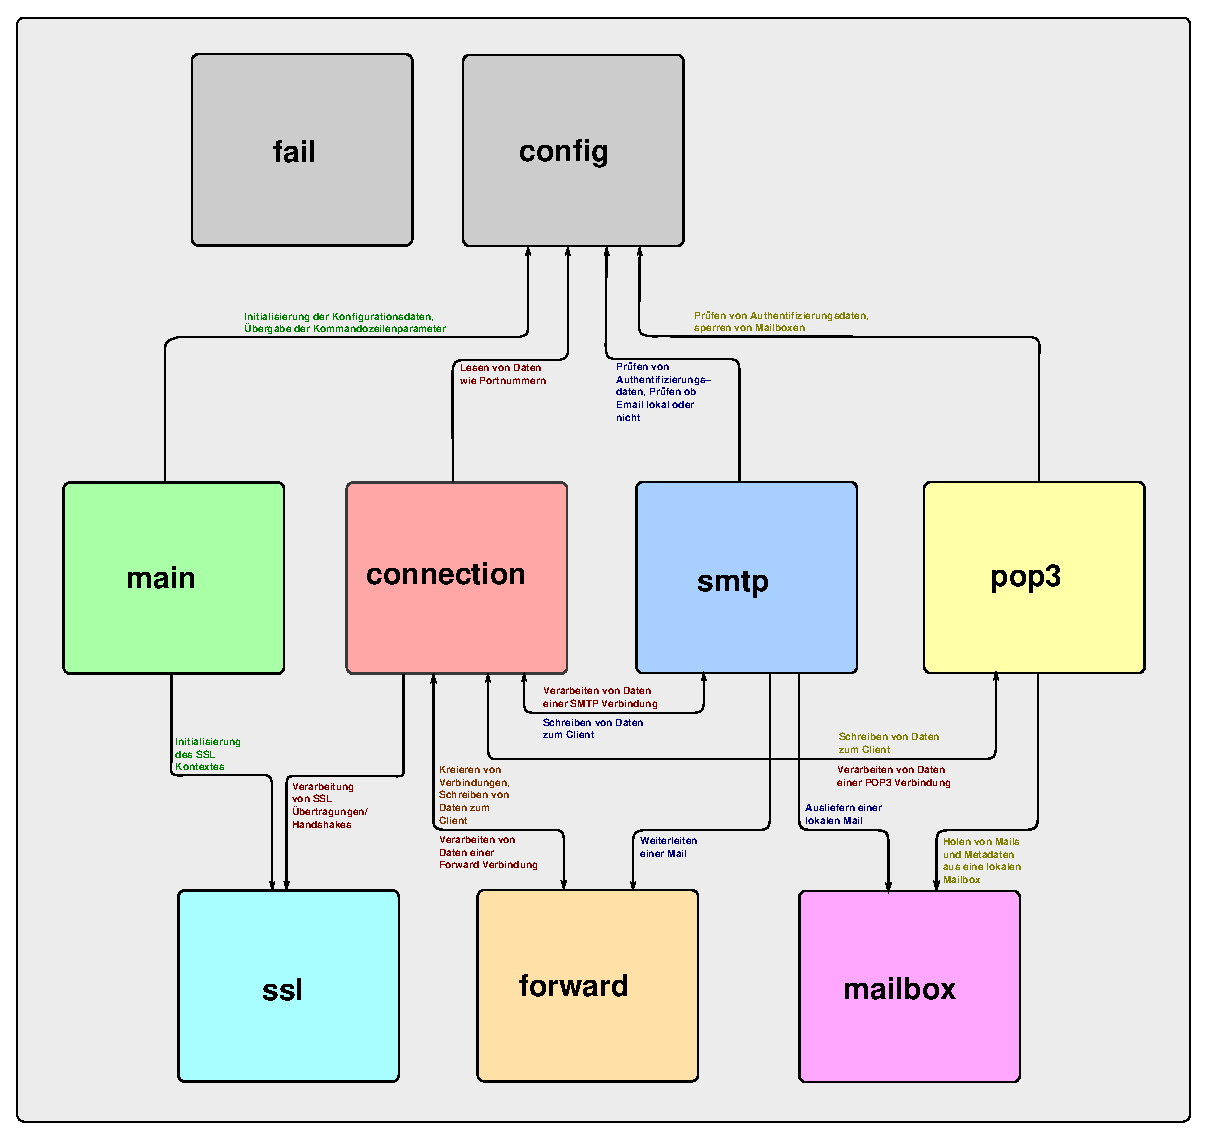
\includegraphics[width=\textwidth]{schema.eps}
    \caption{Modulschema}
    \label{fig:schema}
  \end{figure}
\end{appendix}
\chapter{Sonstiges}
\section{Lizenz}
Copyright (C) 2008, 2009 Jan Losinski

This program is free software; you can redistribute it and/or modify it under
the terms of the GNU General Public License as published by the Free Software 
Foundation; either version 3 of the License, or (at your option) any later 
version.

This program is distributed in the hope that it will be useful, but WITHOUT ANY 
WARRANTY; without even the implied warranty of MERCHANTABILITY or FITNESS FOR A 
PARTICULAR PURPOSE. See the GNU General Public License for more details.

You should have received a copy of the GNU General Public License along with 
this program; if not, see <\url{http://www.gnu.org/licenses/}>.

In addition, as a special exception, the copyright holders give
permission to link the code of portions of this program with the
OpenSSL library under certain conditions as described in each
individual source file, and distribute linked combinations
including the two.

You must obey the GNU General Public License in all respects
for all of the code used other than OpenSSL.  If you modify
file(s) with this exception, you may extend this exception to your
version of the file(s), but you are not obligated to do so.  If you
do not wish to do so, delete this exception statement from your
version.  If you delete this exception statement from all source
files in the program, then also delete it here.

\end{document}
